\subsection{Colorchecker [from Specim scanner]}

White correction of specim scanner is shown in Figure \ref{fig:wc-specim-scanner}. 
The white correction is done by using a white reference and a dark reference. 

Script for white correction is shown in Code \ref{code:wc-specim-scanner}.

\begin{figure}[H]
    \centering
    \caption{White correction of specim scanner}
    \label{fig:wc-specim-scanner}
    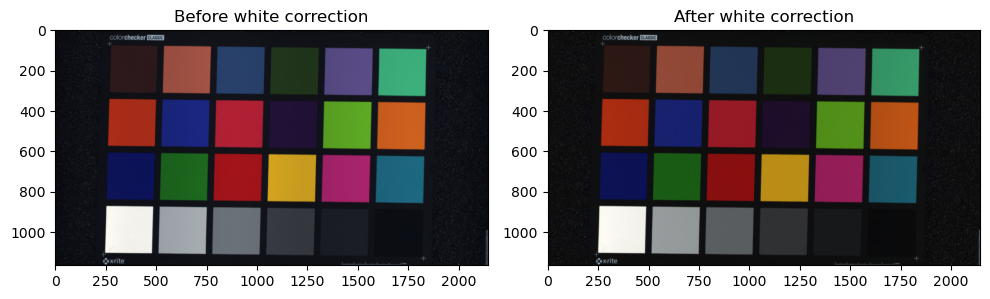
\includegraphics[width=0.75\textwidth]{./fig-task1/specium-scanner.png}
\end{figure}

Spectra of white corrected image is shown in Figure \ref{fig:wc-specim-scanner-spectra}.

\begin{figure}[H]
    \centering
    \caption{Spectra of white corrected image}
    \label{fig:wc-specim-scanner-spectra}
    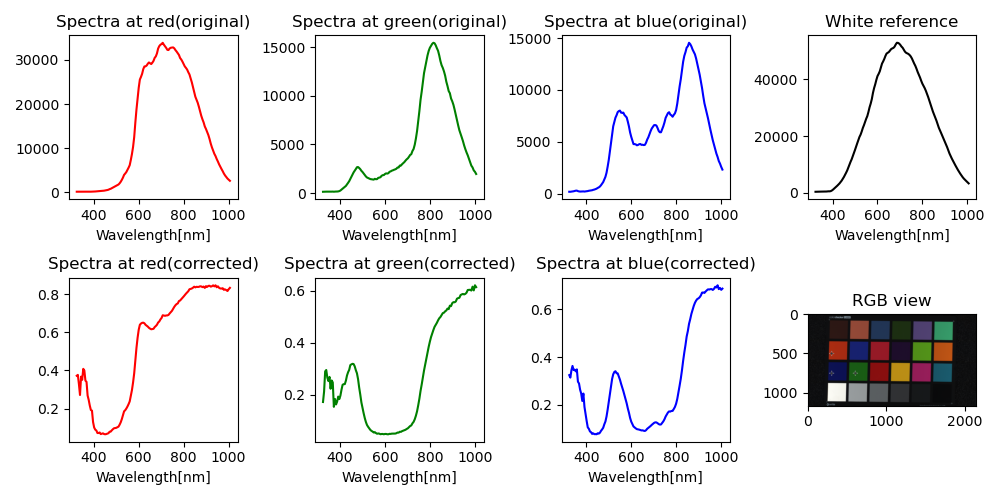
\includegraphics[width=0.75\textwidth]{./fig-task1/wc-specim-scanner-spectra.png}
\end{figure}

\subsection{Color Checker 2 lamps + White Sample 2 lamps}

\subsubsection{SpecimIQ}

White correction of SpecimIQ is shown in Figure \ref{fig:wc-specimiq-large}.

\begin{figure}[H]
    \centering
    \caption{White correction of SpecimIQ with large reference}
    \label{fig:wc-specimiq-large}
    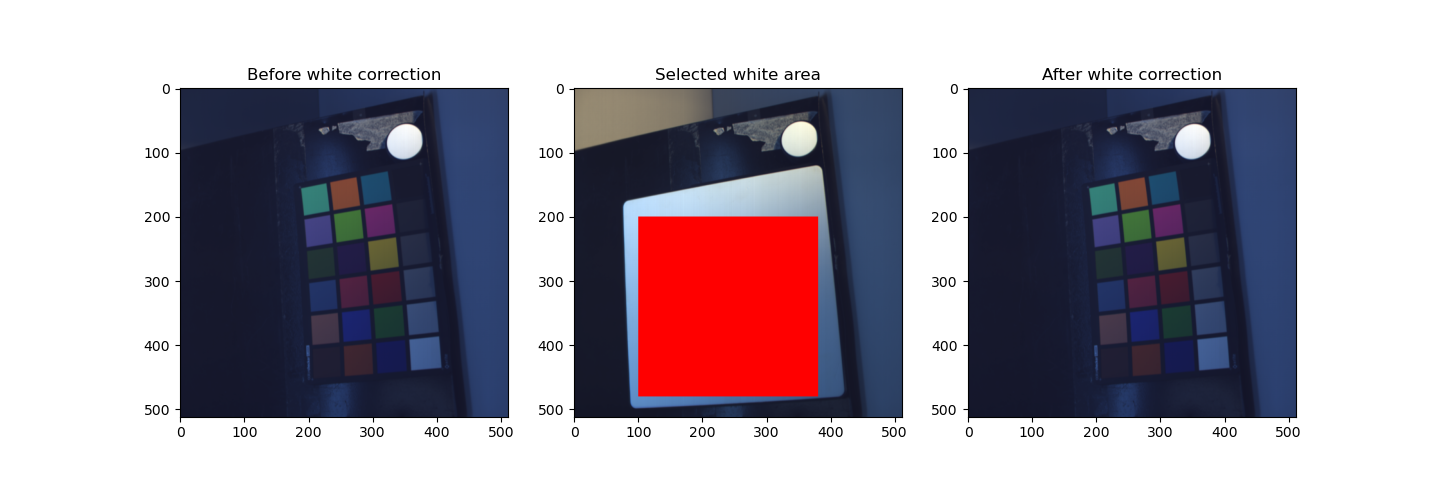
\includegraphics[width=0.75\textwidth]{./fig-task1/wc-specimiq-large.png}
\end{figure}

Spectra of white corrected image is shown in Figure \ref{fig:wc-specimiq-large-spectra}.

\begin{figure}[H]
    \centering
    \caption{Spectra of white corrected image}
    \label{fig:wc-specimiq-large-spectra}
    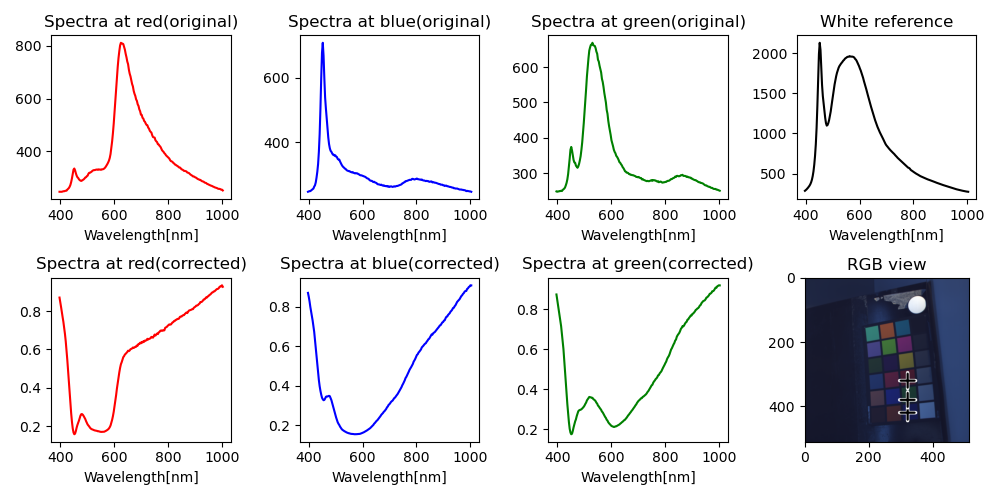
\includegraphics[width=0.75\textwidth]{./fig-task1/wc-specimiq-large-spectra.png}
\end{figure}

Figures were generated with the script shown in Code \ref{code:wc-specimiq-large}.

\subsubsection{Nuance camera}
White correction of nuance camera is shown in Figure \ref{fig:wc-nuance-camera-large}.

\begin{figure}[H]
    \centering
    \caption{White correction of nuance camera with large reference}
    \label{fig:wc-nuance-camera-large}
    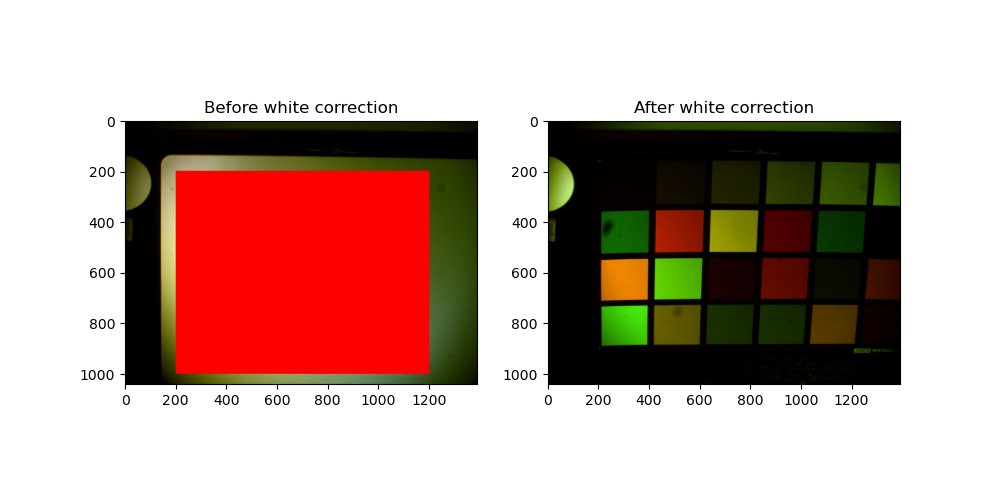
\includegraphics[width=0.75\textwidth]{./fig-task1/wc-nuance-large.png}
\end{figure}

Spectra of white corrected image is shown in Figure \ref{fig:wc-nuance-camera-large-spectra}.

\begin{figure}[H]
    \centering
    \caption{Spectra of white corrected image}
    \label{fig:wc-nuance-camera-large-spectra}
    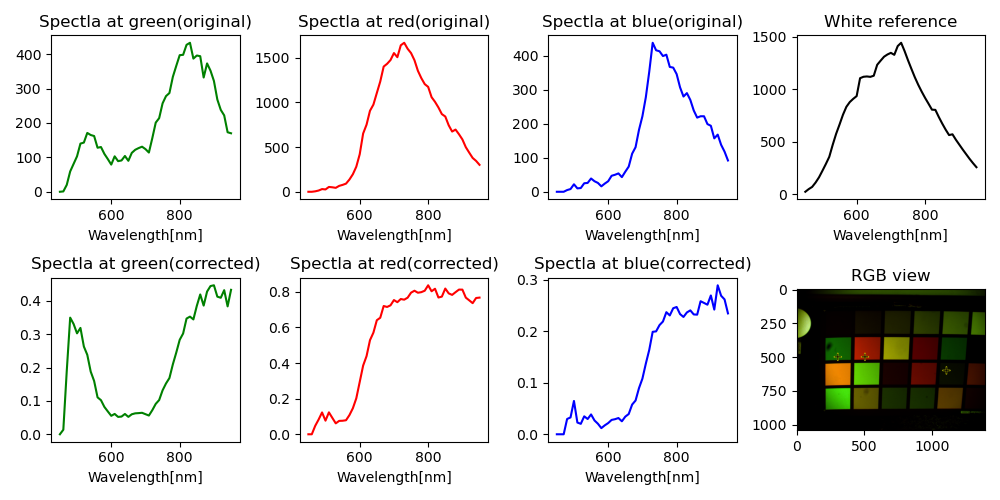
\includegraphics[width=0.75\textwidth]{./fig-task1/wc-nuance-spectra-large.png}
\end{figure}

Nuance image was loaded with the script shown in Code \ref{code:load-nuance}.
Figures were generated with the script shown in Code \ref{code:wc-nuance-large}.


\subsection{Color Checker 2 lamps using left and right white samples inside the image}

\subsubsection{SpecimIQ}
White correction of SpecimIQ is shown in Figure \ref{fig:wc-specimiq-small}.

\begin{figure}[H]
    \centering
    \caption{White correction of SpecimIQ}
    \label{fig:wc-specimiq-small}
    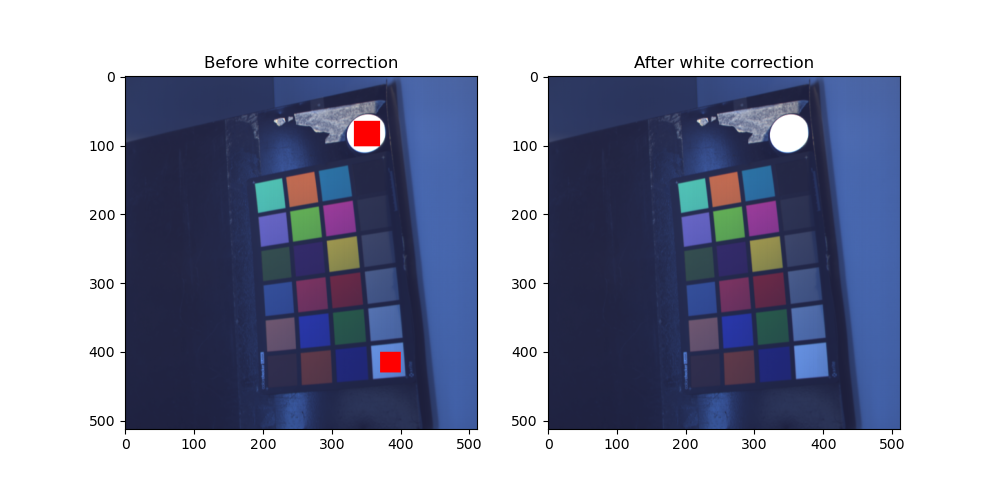
\includegraphics[width=0.75\textwidth]{./fig-task1/wc-specimiq-small.png}
\end{figure}

Spectra of white corrected image is shown in Figure \ref{fig:wc-specimiq-small-spectra}.

\begin{figure}[H]
    \centering
    \caption{Spectra of white corrected image}
    \label{fig:wc-specimiq-small-spectra}
    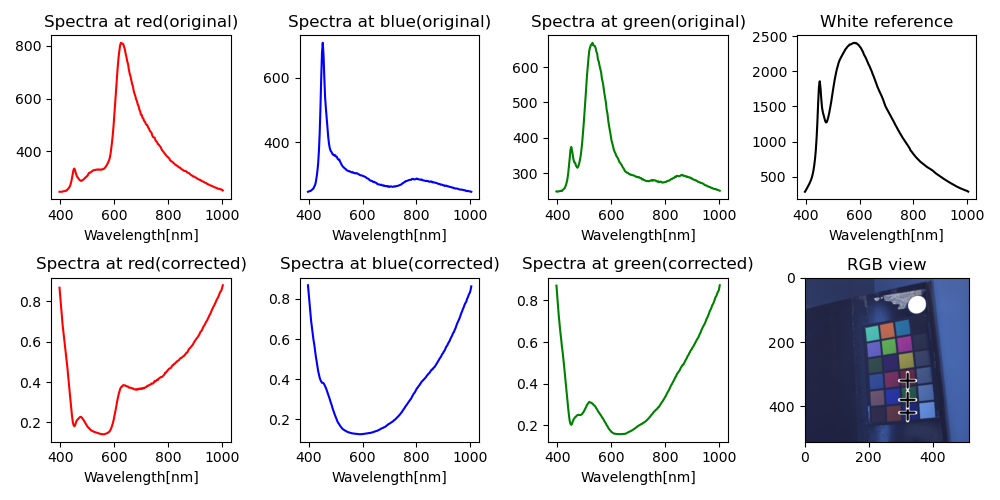
\includegraphics[width=0.75\textwidth]{./fig-task1/wc-specimiq-small-spectra.png}
\end{figure}

Figures were generated with the script shown in Code \ref{code:wc-specimiq-small}.


\subsubsection{Nuance camera}

White correction of nuance camera is shown in Figure \ref{fig:wc-nuance-camera-small}.

\begin{figure}[H]
    \centering
    \caption{White correction of nuance camera}
    \label{fig:wc-nuance-camera-small}
    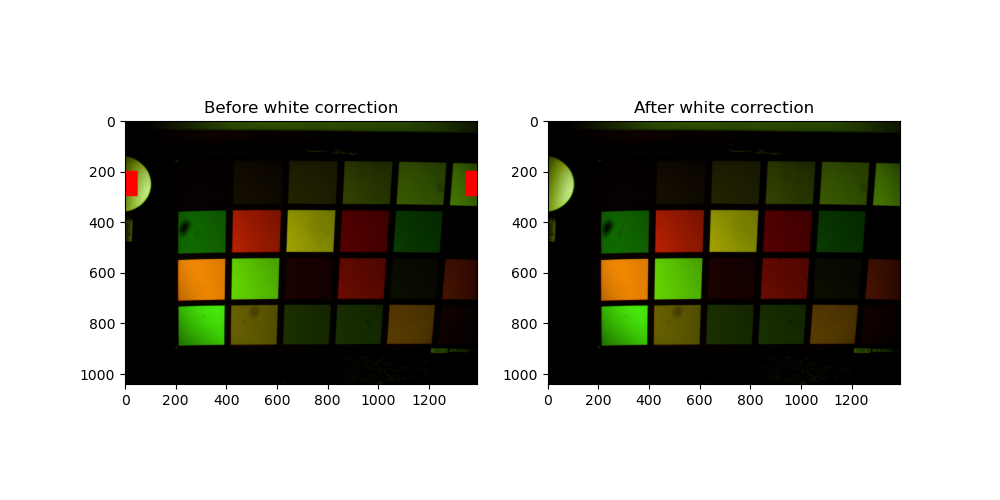
\includegraphics[width=0.75\textwidth]{./fig-task1/wc-nuance-small.png}
\end{figure}

Spectra of white corrected image is shown in Figure \ref{fig:wc-nuance-camera-small-spectra}.

\begin{figure}[H]
    \centering
    \caption{Spectra of white corrected image}
    \label{fig:wc-nuance-camera-small-spectra}
    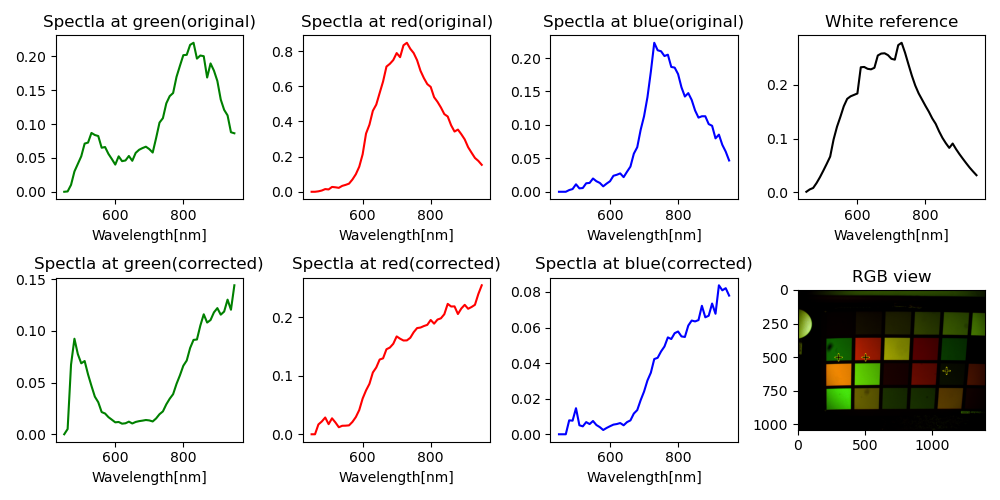
\includegraphics[width=0.75\textwidth]{./fig-task1/wc-nuance-spectra-small.png}
\end{figure}

Nuance image was loaded with the script shown in Code \ref{code:load-nuance}.
Figures were generated with the script shown in Code \ref{code:wc-nuance-small}.


\subsection{Tunable light source}
White correction of tunable light camera is shown in Figure \ref{fig:wc-tunable}.

\begin{figure}[H]
    \centering
    \caption{White correction of tunable light source}
    \label{fig:wc-tunable}
    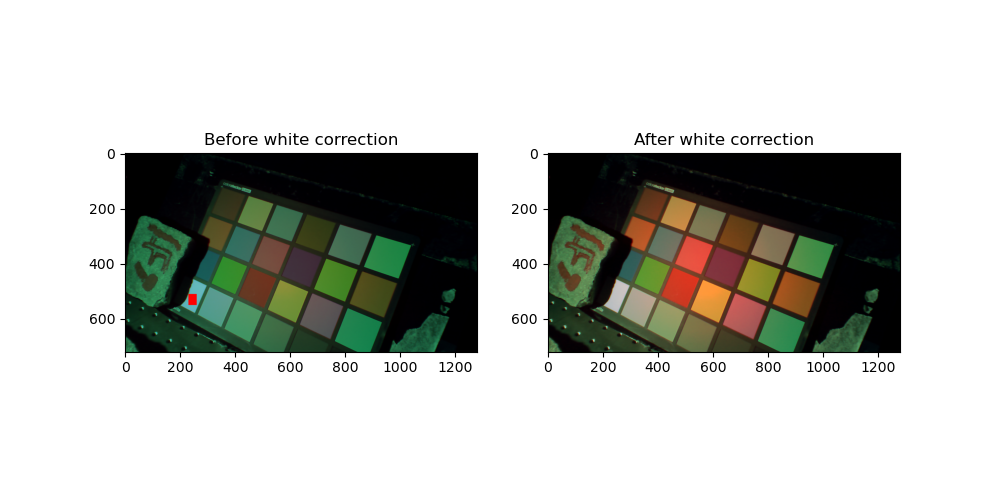
\includegraphics[width=0.75\textwidth]{./fig-task1/wc-tunable.png}
\end{figure}

Spectra of white corrected image is shown in Figure \ref{fig:wc-tunable-spectra}

\begin{figure}[H]
    \centering
    \caption{Spectra of white corrected image}
    \label{fig:wc-tunable-spectra}
    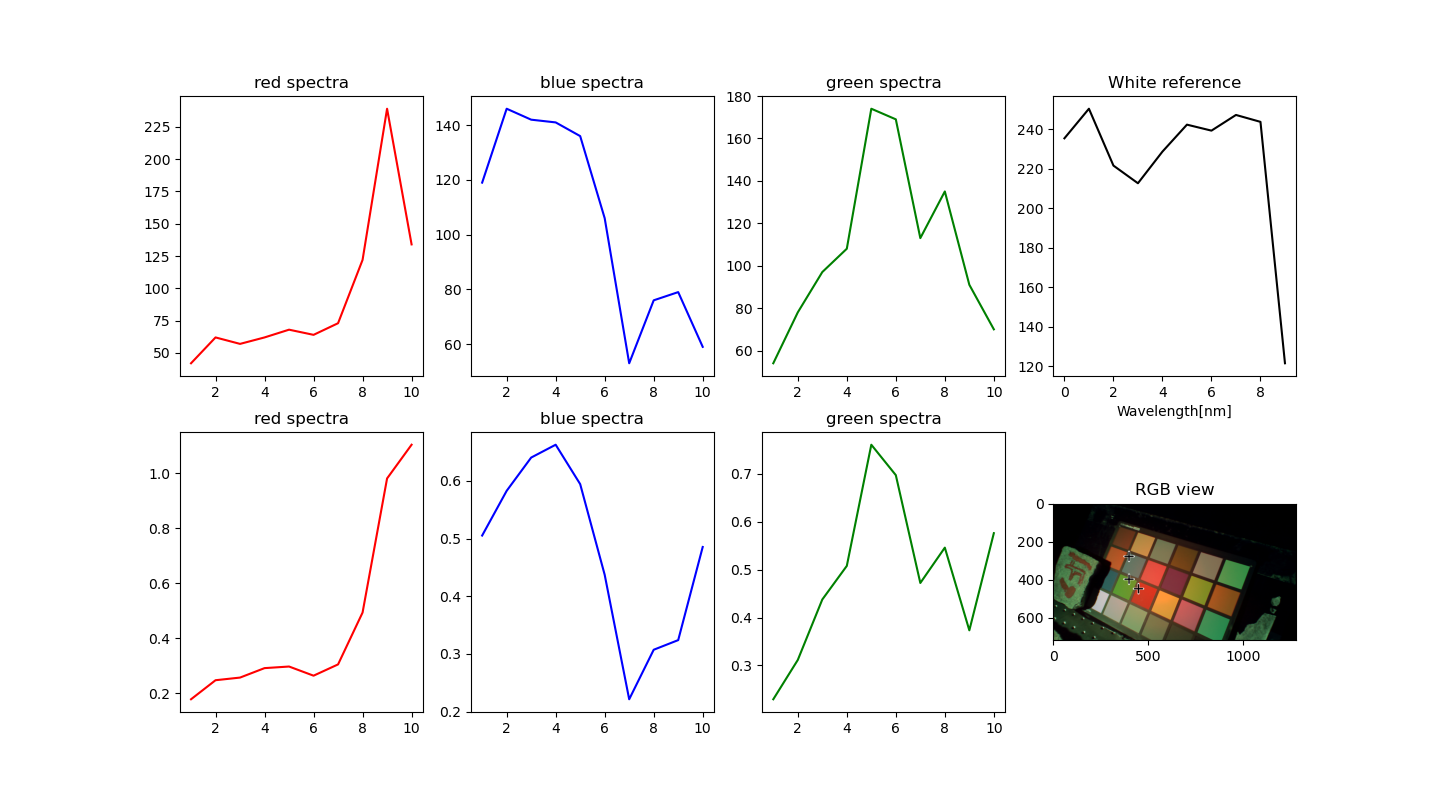
\includegraphics[width=0.75\textwidth]{./fig-task1/wc-tunable-spectra.png}
\end{figure}

Nuance image was loaded with the script shown in Code \ref{code:load-tunable}.
Figures were generated with the script shown in Code \ref{code:wc-tunable}.

